\chapter{Conclusion}

%%%%%%%%%%%%%%%%%%%%%%%%%%%%%%%%%%%%%%%%%%%%%%%%%%%%%%%%%%%%%%%%%%%%%%%%%%%%%%%%%%%%%%%%%%%%%%%%%%%%%%%%%%%%%%%%%%%%%%%%%%%

\section{Bilan}
L'objectif du projet \textit{Virtual-Vertigo} était de réaliser un exercice pour combattre la peur du vide en utilisant des \textit{Google CardBoard} pour visualiser un déplacement dans un monde virtuel. Celui-ci est constitué d'une planche reliant deux immeubles. La personne doit traverser cette planche pour atteindre l'immeuble d'en face sans "chuter". \\

Les éléments suivants ont été mis en place afin d'avoir une simulation opérationnelle :

\begin{itemize}
\item La modélisation de deux scènes virtuelles 3D constituées d'une planche reliant deux immeubles. \\
Cette scène est affichée sur une page Web en utilisant le \textit{Framework X3DOM} permettant d'afficher des scènes 3D. Les scènes ont été modélisées en utilisant des logiciels 3D \textit{Blender et Cinema4D}.
\begin{figure}[H]
\centering
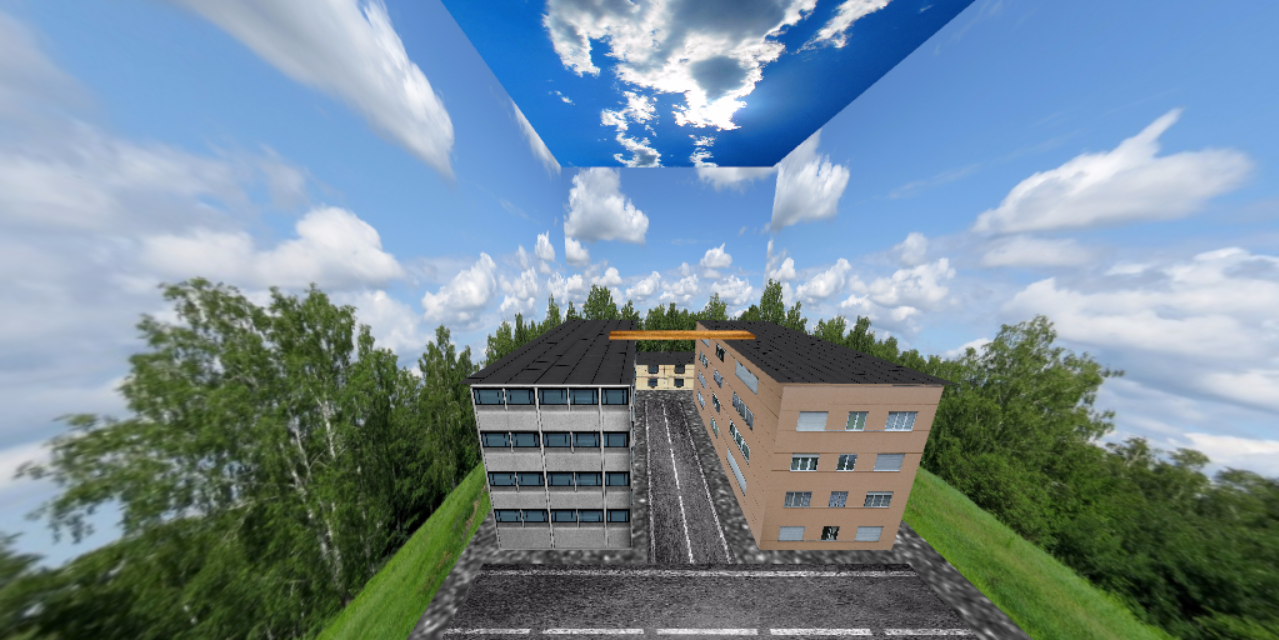
\includegraphics[scale=0.17]{VueBasique2.png}
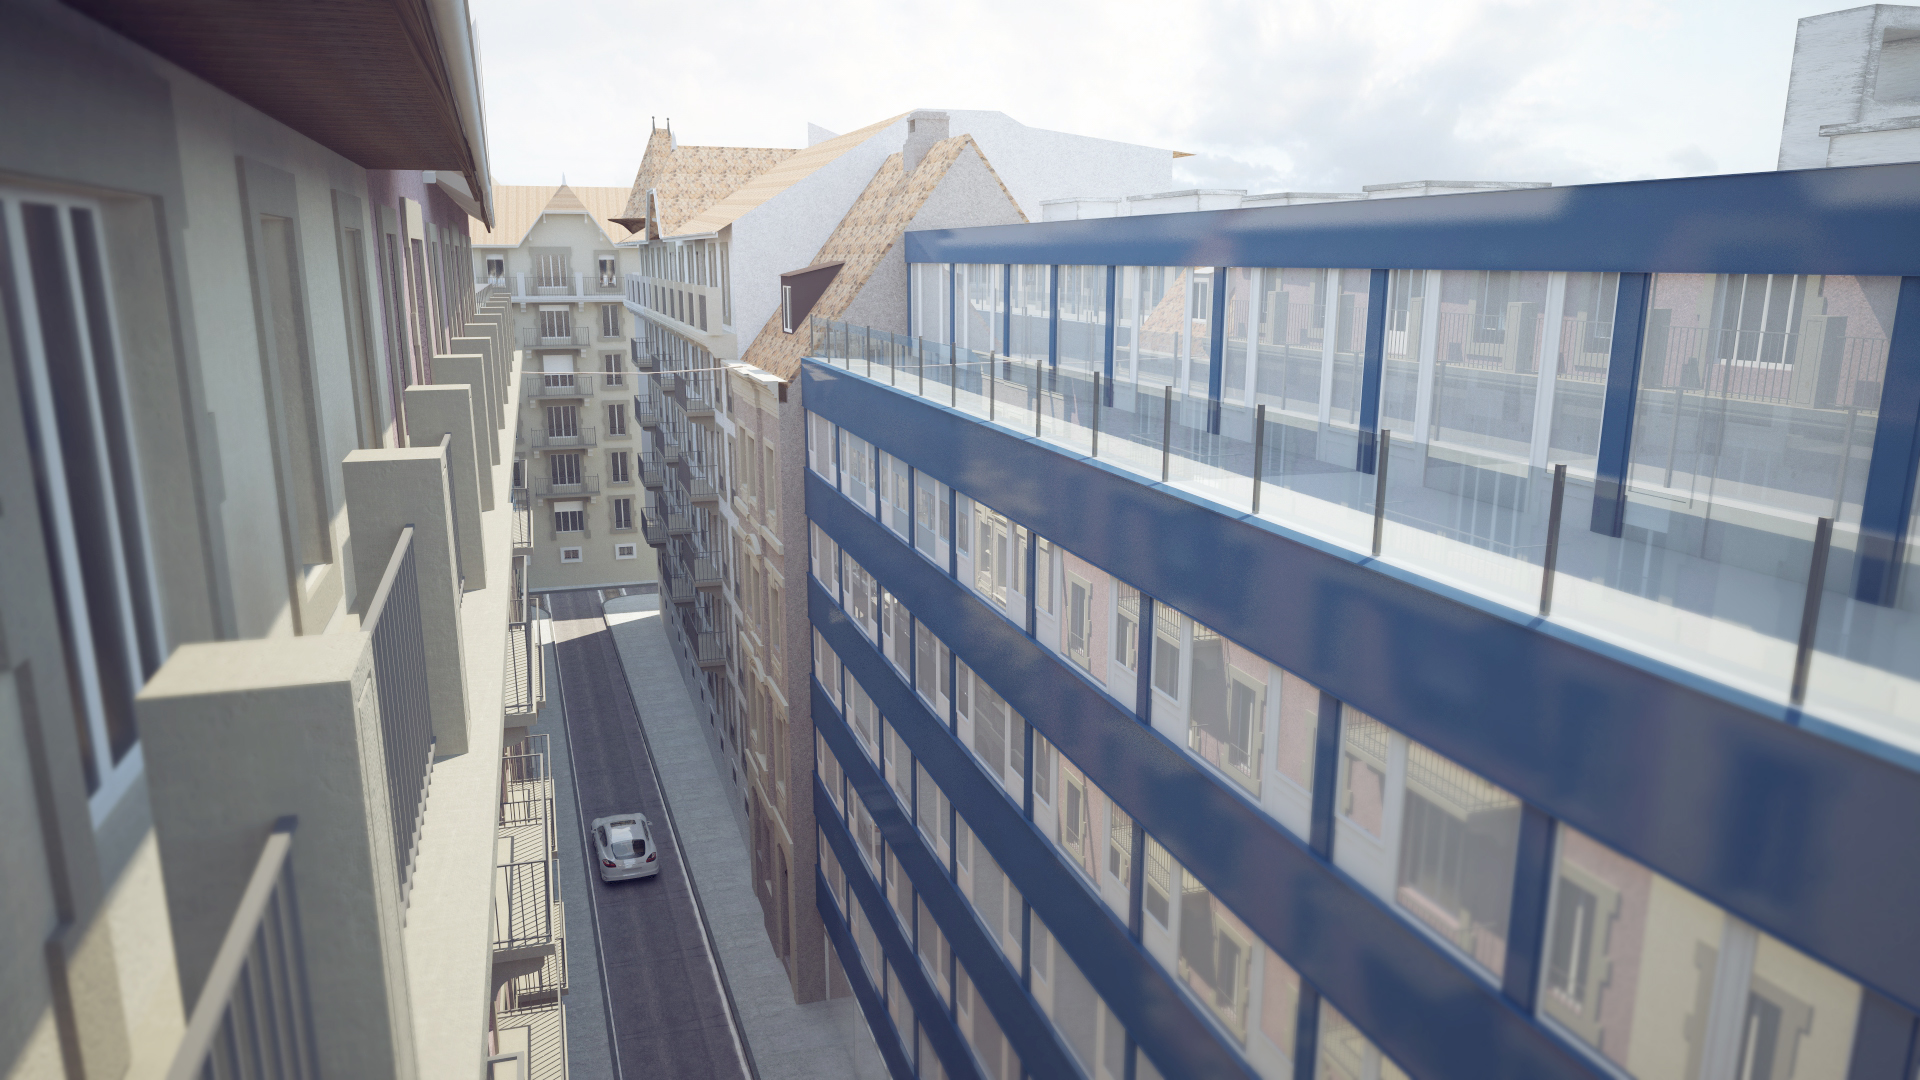
\includegraphics[scale=0.07]{Vue_balcon2_ok.jpg}
\caption{\label{vue} Illustration des scènes virtuelles 3D créées}
\end{figure}

\item La mise en place du \textit{serveur Web Virtual-Vertigo} servant de pont entre le \textit{Kinect version 1} et les clients HTML (le \textsf{smartphone} et le PC). \\
Ce serveur utilise \textit{NodeJS} avec les \textit{modules ExpressJS et Socket.io}.

\item La création d'un \textit{projet Visual Studio} pour le \textit{Kinect} pour la capture des données de positions (articulations du squelette et orientations des mains) et de les transmettre au \textit{serveur Web Virtual-Vertigo} en utilisant SocketIOC\#.
\begin{figure}[H]
\centering
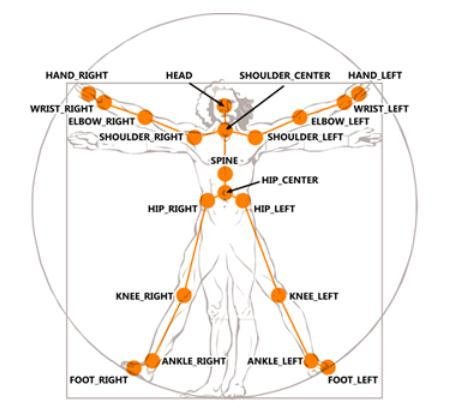
\includegraphics[scale=0.5]{squelette.jpg}
\caption{Illustration des articulations du squelette capturées par le \textit{Kinect v1}}
\end{figure}

\item La création d'un personnage 3D réaliste avec \textit{MakeHuman}.\\
Ce personnage n'est pas utilisé dans la version finale car il est devenu rigide lors de l'exportation en X3D depuis \textit{Blender}.
\begin{figure}[H]
\centering
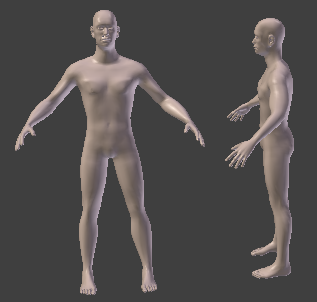
\includegraphics[scale=0.4]{PersonnageRealiste.png}
\caption{Illustration du personnage réaliste créé}
\end{figure}

\item La création d'un client HTML pour le \textsf{smartphone} contenant une vue stéréoscopique de la réalité virtuelle utilisant \textit{X3DOM}. \\ Un problème avec le positionnement des textures visible sur la figure~\ref{vueSmartphone} persiste.
\begin{figure}[H]
\centering
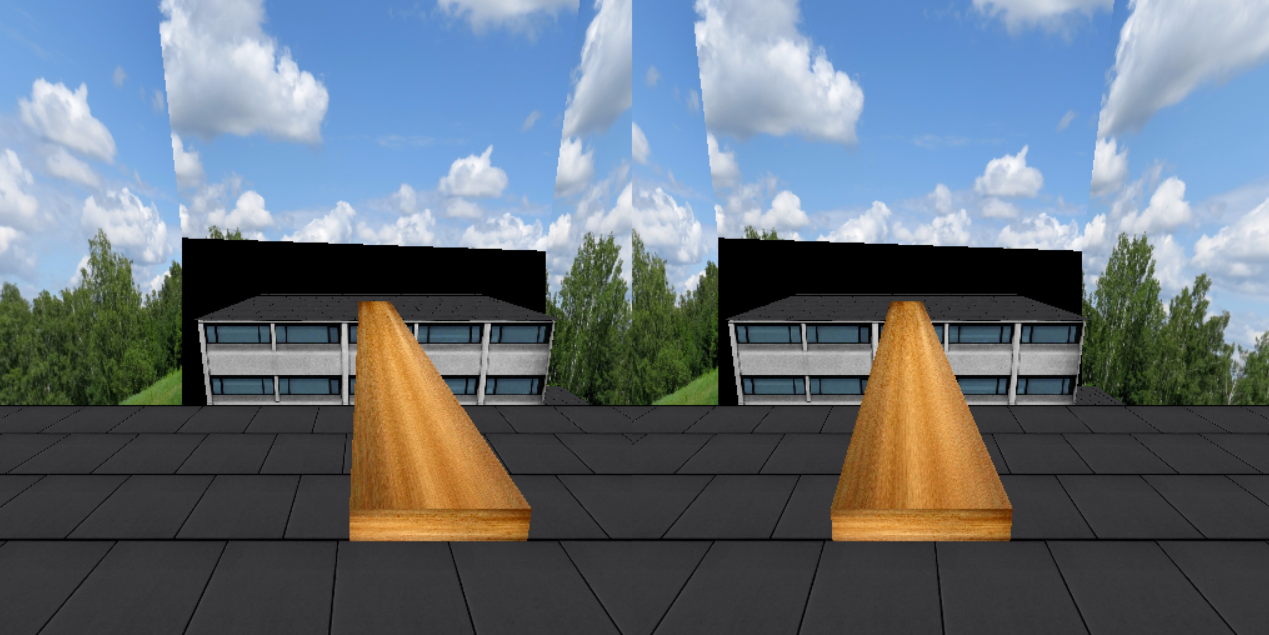
\includegraphics[scale=0.15]{VueSmartphone.png}
\caption{\label{vueSmartphone} Illustration de la vue stéréoscopique sur le \textsf{smartphone}}
\end{figure}

\item La création d'un client HTML pour le PC pour afficher la simulation sur un écran standard toujours avec \textit{X3DOM}.
\item La construction d'un squelette 3D dans la réalité virtuelle afin de l'animer. \\
Des sphères sont placées sur les articulations et des cylindres relient les articulations voisines.
\item Le déplacement (en \textsf{JavaScript}) de la personne sur la planche dans la réalité virtuelle en fonction de la position de la tête capturée par le \textit{Kinect version 1}.
\begin{figure}[H]
\centering
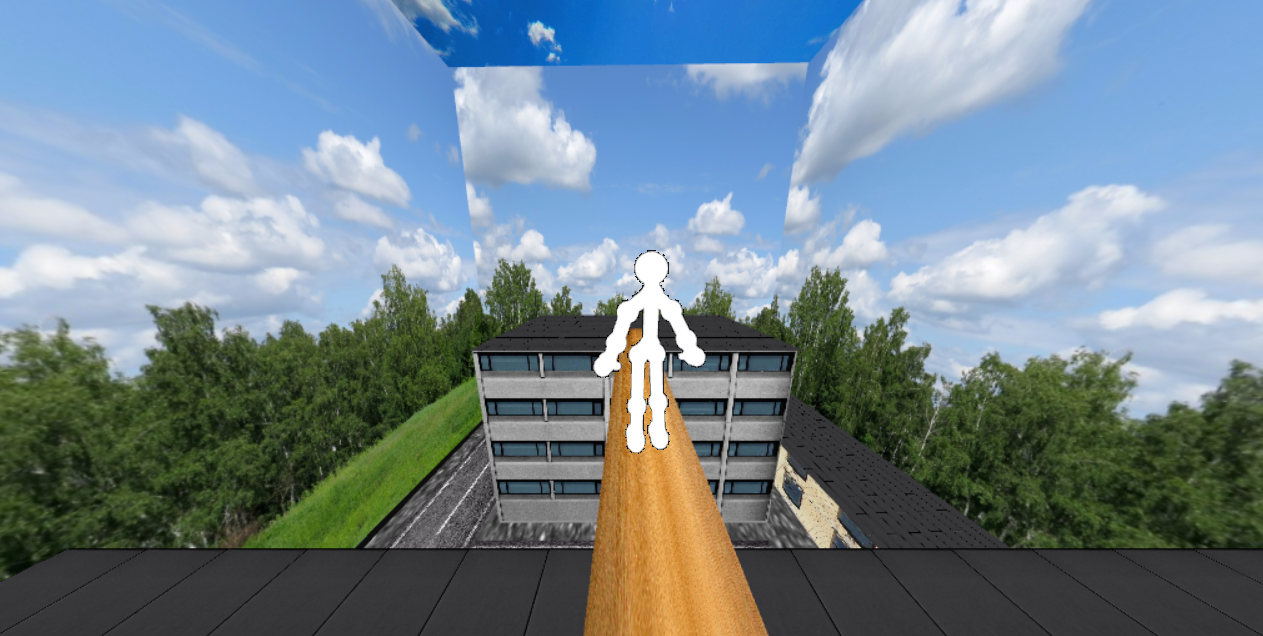
\includegraphics[scale=0.15]{Deplacement.png}
\caption{\label{Deplacement} Illustration du déplacement du squelette 3D dans la réalité virtuelle}
\end{figure}

\item L'animation des membres du squelette 3D en fonction des données capturée par le \textit{Kinect version 1}. \\
Cela nécessitait de positionner et calculer l'angle entre deux articulations voisines du squelette.
\item L'adaptation de la scène virtuelle en fonction de l'orientation de la tête. \\
Cette orientation est détectée via les accéléromètres du \textsf{smartphone}.
\item L'ajout d'effets afin de rendre la simulation plus réaliste : \\
\begin{itemize}
\item une planche réelle sur le sol.
\item un bruit ambiant en utilisant un casque sans fil.
\item une animation de "chute" lorsque l'utilisateur n'a plus les pieds sur la planche. \\
La simulation recommence après une "chute" ou lorsque l'utilisateur est arrivé à l'extrémité de la planche.
\end{itemize}
\end{itemize}

La figure~\ref{simulation} montre à gauche un camarade de diplôme, \textsc{M. Vasco Marques}, effectuant la simulation du projet et à droite la vue affichée sur les \textit{Google CardBord} lors de sa simulation.
\begin{figure}[H]
\centering
	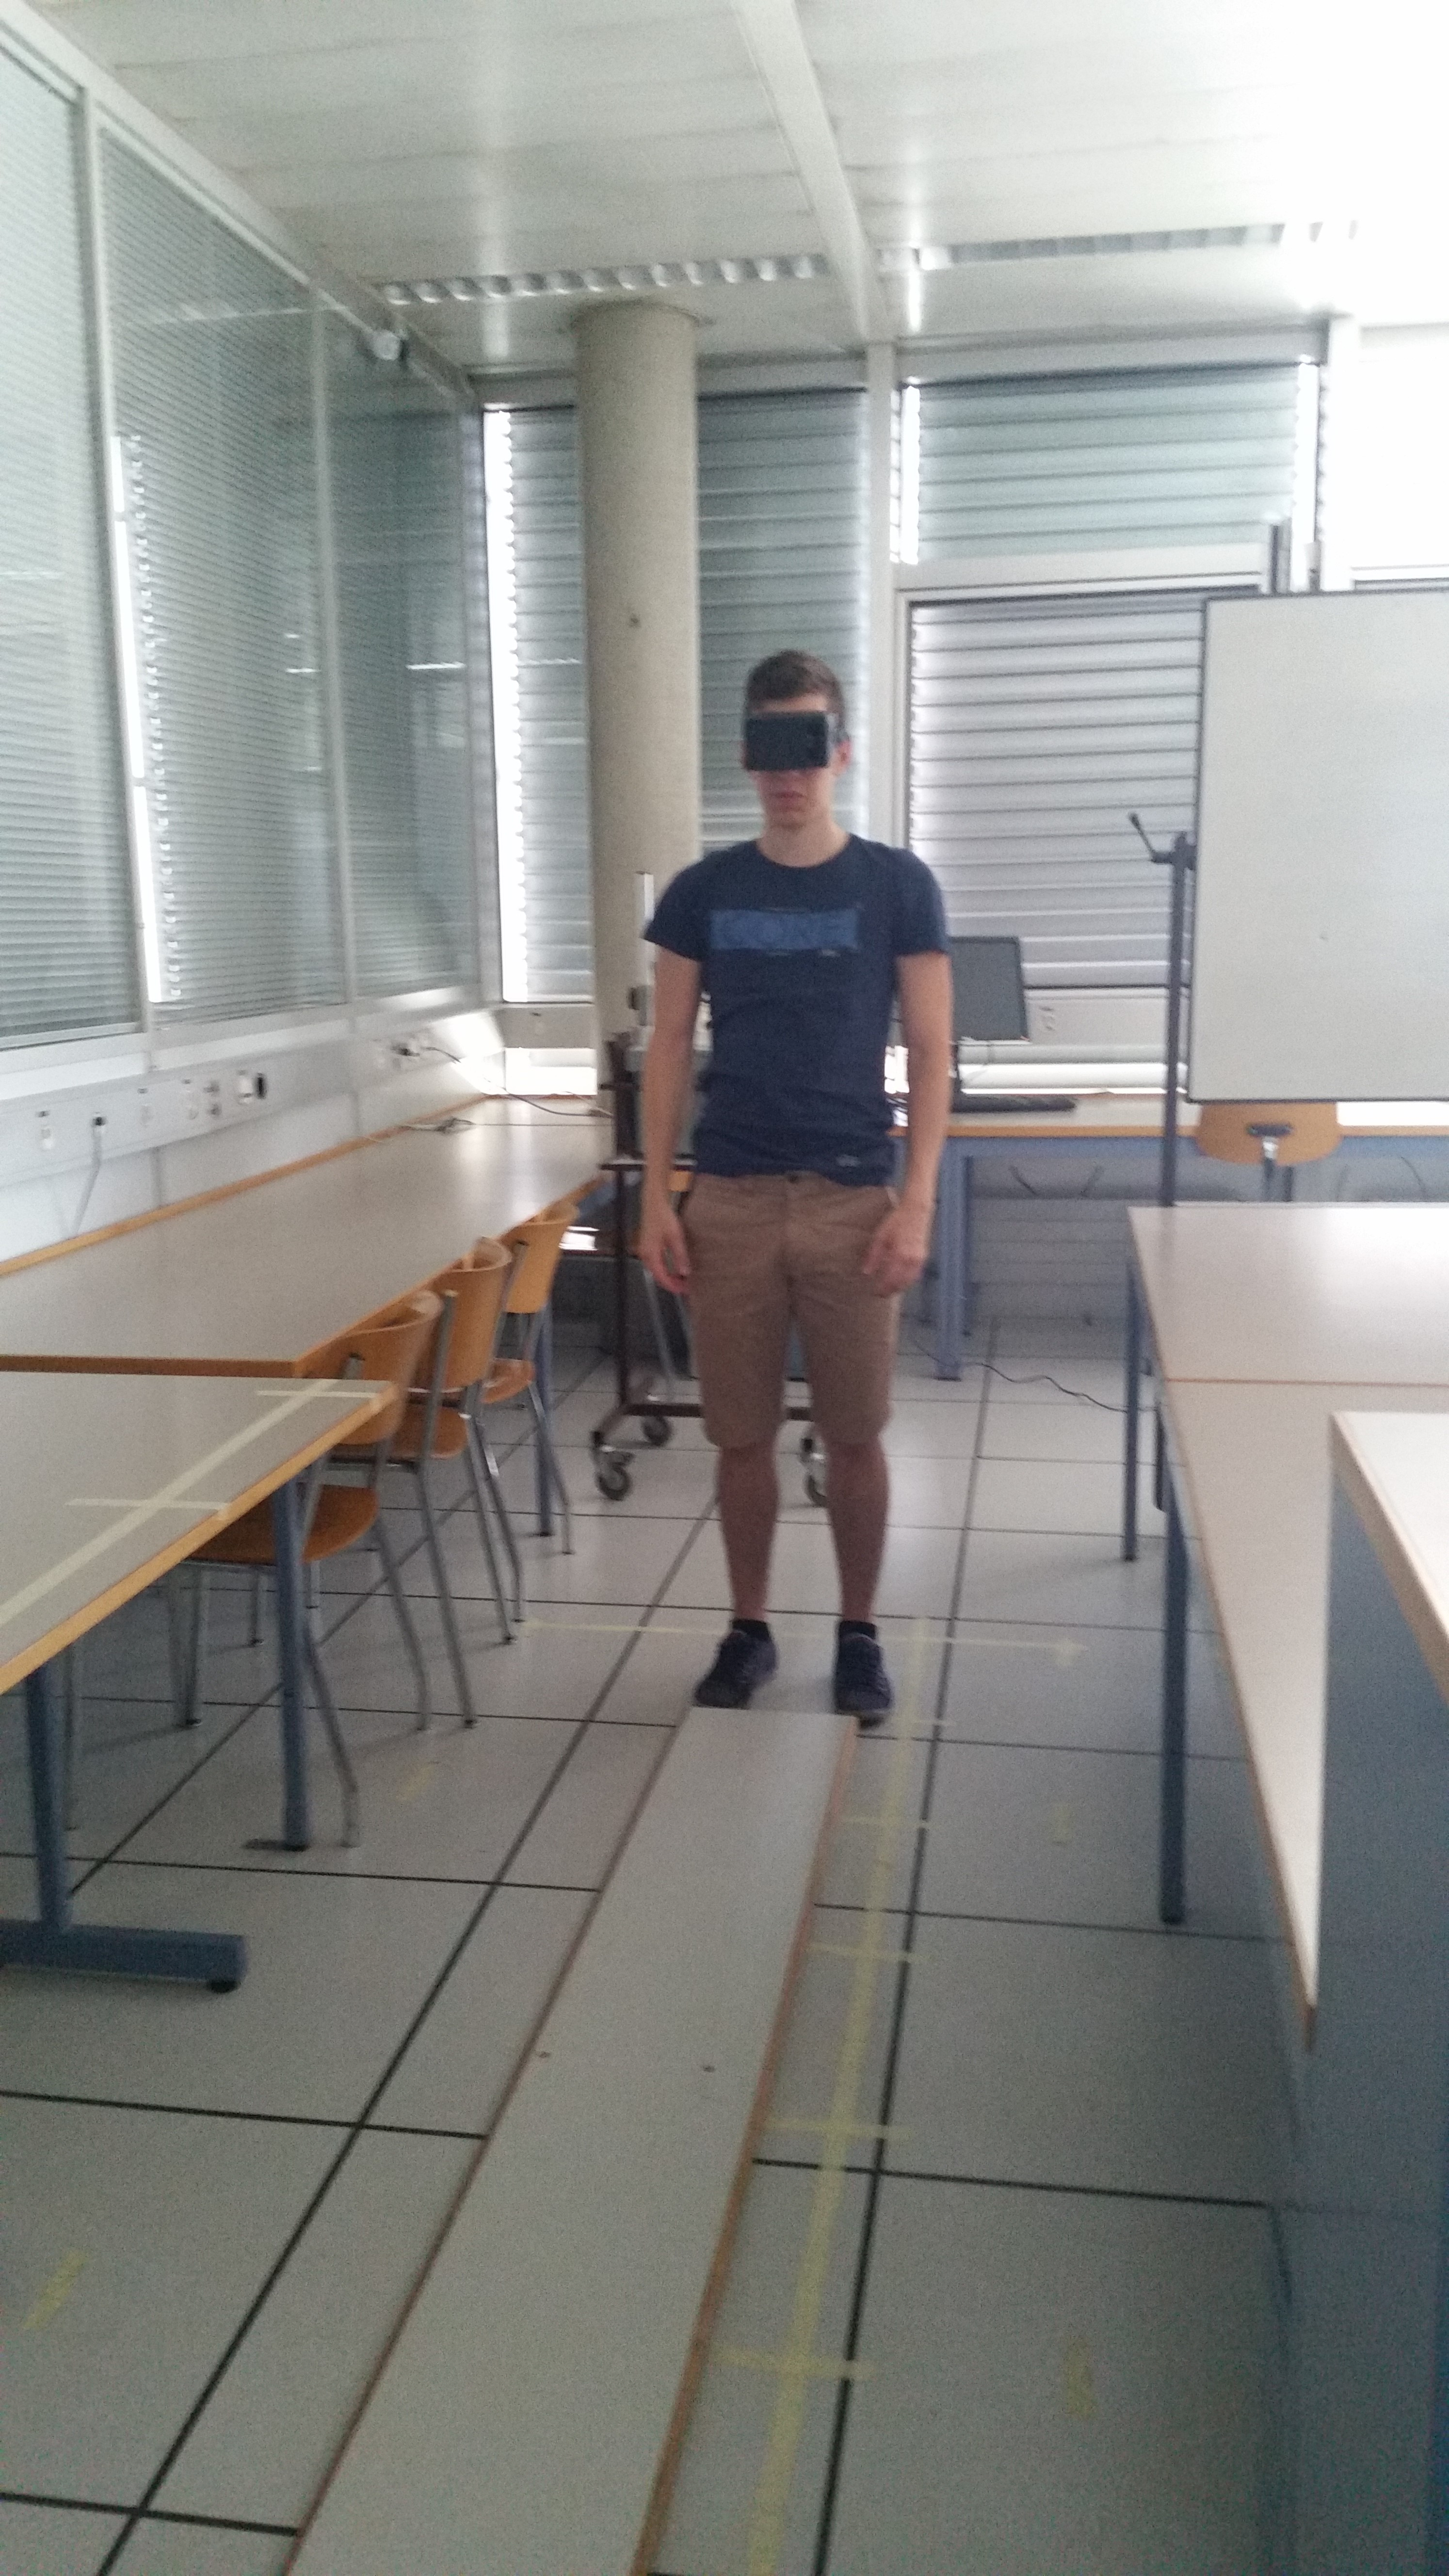
\includegraphics[scale=0.03]{vueReelle1.jpg}
	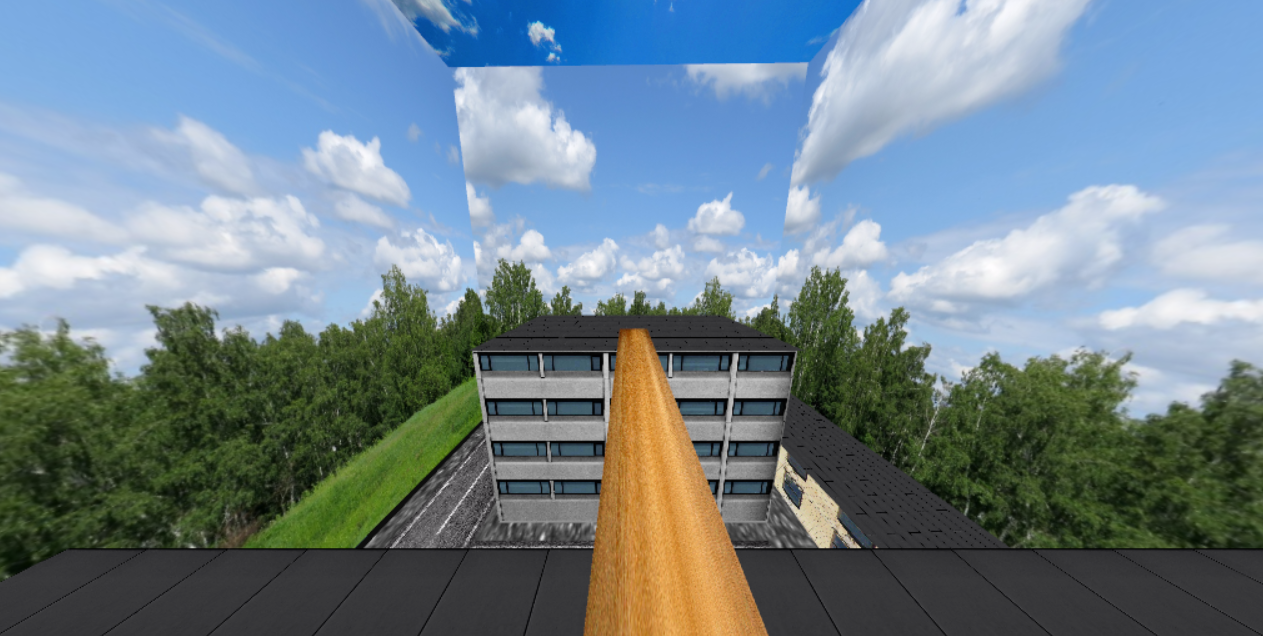
\includegraphics[scale=0.2]{vueBasiqueTextures.png}
\caption{\label{simulation} Simulation de Virtual-Vertigo}
\end{figure}

A la fin de ce travail de Bachelor, une simulation complète est opérationnelle. Il est possible de porter les \textit{Google CardBoard} et de faire la simulation en ayant une planche posée sur le sol et un casque \textsf{bluetooth} diffusant un bruit ambiant enregistré. Cependant quelques problèmes n'affectant pas la simulation persistent: 
\begin{enumerate}
\item le décalage de la vue lorsque le \textsf{smartphone} prend le relais pour l'orientation de la vue en fonction de la tête;
\item le positionnement non optimal des textures dans la vue affichée sur le \textsf{smartphone};
\item la visualisation  non optimale des membres qui parfois ne s'affichent pas alors que la personne tient ses mains bien devant elle (ils paraissent plus petits en virtuel que dans la réalité).
\end{enumerate}

%%%%%%%%%%%%%%%%%%%%%%%%%%%%%%%%%%%%%%%%%%%%%%%%%%%%%%%%%%%%%%%%%%%%%%%%%%%%%%%%%%%%%%%%%%%%%%%%%%%%%%%%%%%%%%%%%%%%%%%%%%%

\section{Améliorations}
Quelques améliorations possibles pour ce projet sont les suivantes :
\begin{itemize}
\item corriger les problèmes persistants 
\item ajouter le reste des effets de réalisme (la montre connectée et le ventilateur)
\item utiliser la \textit{Kinect v2} afin d'avoir plus de précisions sur l'orientation des mains
\item utiliser le \textsf{smartphone} pour lancer l'effet sonore au lieu du casque sans fil
\item trouver d'autres effets de réalisme pour augmenter l'immersion de la personne 
\item améliorer les \textit{Google CardBoard} afin de les rendre plus esthétiques et plus agréable à porter
\item étudier la possibilité d'un composant disponible sur le \textsf{smartphone} en remplacement de la \textit{Kinect}
\end{itemize} 

\section{Perspectives}
Afin de pouvoir vraiment utiliser le projet \textit{Virtual-Vertigo} dans un contexte médical, il faudrait contacter un psychologue ou un spécialiste pour évaluer le projet. Cette évaluation permettrait de savoir si l'approche choisie pour ce projet est vraiment utile pour aider les personnes ayant le vertige. En cas de succès auprès d'un spécialiste, le projet pourrait être lancé avec une \textsf{startup} et serait distribué dans la médecine thérapeutique. Une autre possibilité de vente serait envisageable. En effet, l'armée ou les services de pompiers pourraient être intéressés par des variantes de \textit{Virtual-Vertigo}. Celles-ci pourraient leur être utile afin de tester ou entraîner leurs nouvelles recrues dans un environnement virtuel similaire à celui de \textit{Virtual-Vertigo}. 

